\documentclass[12pt]{article}
\usepackage[shortlabels]{enumitem}
\usepackage{float}
\usepackage{xcolor}
\usepackage[a4paper, top=1.5cm, bottom=1.5cm, left=2cm, right=2cm]{geometry}
\usepackage{parskip}
\usepackage{setspace}
\usepackage{lmodern}
\usepackage[T1]{fontenc}
\usepackage[brazil]{babel}
\usepackage{hyperref}
\usepackage{graphicx}
\usepackage{amsmath}
\usepackage{amssymb}
\usepackage{amsfonts}
\usepackage{dsfont}
\usepackage{float}
\title{Lista 2 - Estatística para Administração - 2025.2}
\begin{document}
\date{}
\maketitle

1) Consiste em realizar afirmações acerca da população a partir da amostra. 
Não podemos realizar inferência baseado em uma amostra gerada por um método não probabilístico. Esse ponto será discutido com maior profundidade quando 
estudarmos o processo inferência estatística. 
\vspace{5px}

2) Determine o valor numérico das seguintes expressões:

\begin{enumerate}[a)] % a), b), c), ...
    \item $\sum\limits_{i = 1}^3 i = 6$ \\
    \item $\sum\limits_{i = 1}^5 i^2 = 55 $ \\
    \item $\sum\limits_{i = 1}^4 \dfrac{1}{i} = \frac{25}{12}$ \\
    \item $\sum\limits_{i = 1}^4 (-1)^{i} = 0$ \\
    \item $\sum\limits_{i = 1}^3 4x = 12x$ \\
    \item $\sum\limits_{i = 1}^n (-1)^{i}$ onde $n$ é par $=0$\\
    \item $\sum\limits_{i = 1}^n (-1)^{i}$ onde $n$ é ímpar $=-1$\\
    \item $\prod\limits_{i=1}^5 (i-1)^2 = 0$\\
    \item $\prod\limits_{i=1}^3 2^i = 64$\\
    \item $\prod\limits_{i=1}^n -1$ onde $n$ é par $=1$\\
    \item $\sum\limits_{x \in \{ 1, 2,5,6,20,10\}} x = 44$ \\ 
    \item $\sum\limits_{s \in \{ 2,4,6,8,10\}}  \dfrac{e^s}{\sum\limits_{m \in \{ 2,4,6,8,10\}} e^m}  = 1$ \\
    \item $\sum\limits_{i=1}^5\sum\limits_{j=1}^3 2^j = 70$
    \item $\sum\limits_{i=1}^5\sum\limits_{j=0}^i 3^{(j-1)} = 542/3$
\end{enumerate}
\vspace{5px}

3) Considere o seguinte conjunto de dados referente a uma pesquisa realizada com estudantes da Praia Vermelha acerca da participação em Empresa Júnior:

\begin{table}[H]
\centering
\begin{tabular}{llll}
\hline
Nome     & Idade & Curso          & E.Junior \\ \hline
Matheus  & 22    & Economia       & 1        \\
Pawel    & 31    & Administração  & 0        \\
Jean     & 29    & Administração  & 1        \\
Janaina  & 18    & Contabilidade  & 1        \\
Leandro  & 19    & Psicologia     & 0        \\
Karolina & 62    & Psicologia     & 0        \\
Katarina & 41    & Administração  & 1        \\
Gilberto & 22    & Economia       & 1        \\
Maya     & 27    & Serviço Social & 1        \\ \hline
\end{tabular}
\end{table}

A a coluna E.Junior indica se o estudante participa ou não de Empresa Júnior. 1 - Sim e 0 Não.

\begin{enumerate}[a)]
    \item $\bar{x}=30,11$. Fornecer apenas a média não é suficiente para entender a variável, pois a média pode ser distorcida pela presença de pontos aberrantes, além de não descrever a variabilidade dos valores assumidos pela variável. 
    \item C\begin{table}[]
\begin{tabular}{llll}
\hline
Curso          & $n_i$ & $f_i$  & $f_{ac}$ \\ \hline
Economia       & 2     & 0,2222 & 0,2222   \\
Administração  & 3     & 0,3333 & 0,5555   \\
Psicologia     & 2     & 0,2222 & 0,7777   \\
Contabilidade  & 1     & 0,1111 & 0,8888   \\
Serviço Social & 1     & 0,1111 & 1        \\
Total          & 9     & 1      &          \\ \hline
\end{tabular}
\end{table}

A variável Curso é qualitativa nominal. A variável Nome também  é qualitativa nominal.
    \item Calcule a médiana da Idade dos participantes. Compare a mediana com a média encontrada na questão a), o que você consegue extrair de informação a partir dessas duas medidas de forma conjunta?
    \item Defina $y$ como a variável que representa os valores da coluna E.Junior. Considera a seguinte métrica 
    $\hat{p}=\dfrac{\displaystyle\sum_{k=1}^{9} y_k}{9} $. Calcule o valor de $\hat{p}$ e diga em palavras o significado de $\hat{p}$.
    \item Defina $x$ como a variável que representa os valores da coluna Idade. Calcule o valor da métrica $\varepsilon = \sum_{i=1}^{9} \dfrac{x_i - \bar{x}}{n}$. O que essa métrica significa em termos práticos?
\end{enumerate}

\end{table}

\vspace{5px}

4) Considere o gráfico a seguir referente à nacionalidade dos estudantes que prestaram o ENEM no ano de 2022. 

\begin{figure}[H]
         \centering
        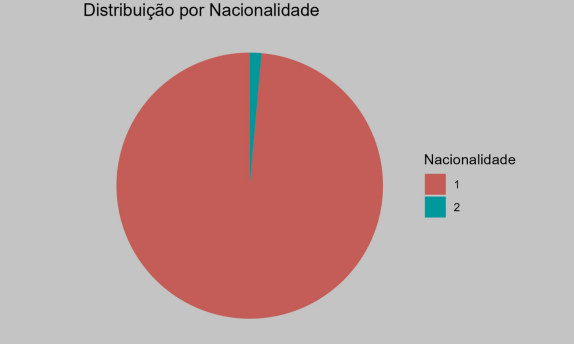
\includegraphics[width=0.4\linewidth]{figures/pizza_1_exercicio.png}
    \end{figure}

Quais problemas você identifica no gráfico acima? Se você tivesse que criar uma visualização para representar esses dados, o que você faria diferente?

\vspace{5px}

5) Considere o gráfico a seguir referente ao acompanhamento de indivíduos com insuficiência cardíaca. 

\begin{figure}[H]
         \centering
        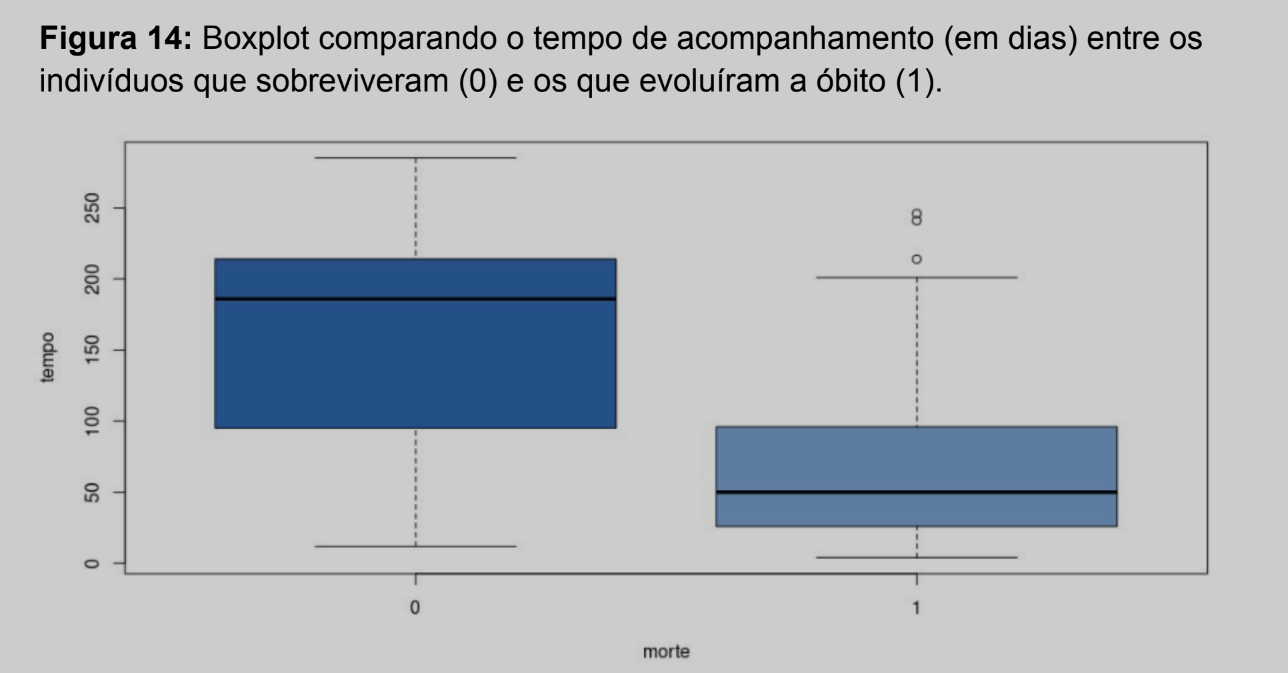
\includegraphics[width=0.6\linewidth]{figures/boxplot_2.png}
    \end{figure}

Interprete o gráfico acima. Quais conclusões podemos tirar a respeito dos pacientes que faleceram em relação aos que não faleceram? 

\vspace{5px}

6) Na matemática é muito comum nos depararmos com potências envolvendo binômios. Por exemplo, no Ensino Médio é muito comum usarmos o resultado: 
$$(x+y)^2 = x^2 + 2xy + y^2$$ 

No entanto, o caso acima é apenas um caso restrito do Teorema Binomial. O Teorema Binomial nos permite expandir qualquer potência de um binômio através da seguinte relação:

$$(x+y)^n = \sum_{k=0}^n  \binom{n}{k} x^{n-k} y^k, $$

onde $\binom{n}{k} = \dfrac{n!}{k!(n-k)!}$

Dado o resultado do Teorema, encontre a expansão do binômio $(a+b)^5$. 

\vspace{5px}

7) Responda as seguintes questões envolvendo o uso do R. 

\begin{enumerate}[a)]
    \item Crie um vetor chamado \textit{idade} e armazene os valores 12, 27, 42, 26, 33, 25, 44, 17, 29, 33 
    \item Crie um vetor chamado \textit{curso} e armazene os valores Adm, Adm, CC, Adm, CC, Adm, Adm, CC, Adm, CC
    \item  Escreva e em seguida execute o comando \textit{table(curso)}. O que você obteve por meio desse comando? 
    \item Escreva e em seguida execute o comando \textit{prop.table(table(curso))}. O que você obteve por meio desse comando? 
    \item Escreva e em seguida execute o comando \textit{mean(idade)}. O que você obteve por meio desse comando? 
    \item Escreva e em seguida execute o comando \textit{median(idade)}. O que você obteve por meio desse comando? 
    \item Escreva e em seguida execute o comando \textit{mode(idade)}. O que você obteve por meio desse comando? (\textcolor{red}{Muita atenção nesse ponto!})
    \item Escreva e em seguida execute o comando \textit{quantile(idade)}. O que você obteve por meio desse comando? 
    \item Escreva e em seguida execute o comando \textit{quantile(idade, 0.6)}. O que você obteve por meio desse comando? 
    \item Escreva e em seguida execute o comando \textit{quantile(idade, 0.05)}. O que você obteve por meio desse comando? 
    \item Escreva e em seguida execute o comando \textit{quantile(idade, 1)}. O que você obteve por meio desse comando? 
    \item Escreva e em seguida execute o comando \textit{quantile(idade, 0)}. O que você obteve por meio desse comando?
    \item Escreva e em seguida execute o comando \textit{min(idade)}. O que você obteve por meio desse comando?
    \item Escreva e em seguida execute o comando \textit{max(idade)}. O que você obteve por meio desse comando?
    \item Escreva e em seguida execute o comando \textit{table(cut(idade, 4))}. O que você obteve por meio desse comando?
    \item Refaça os exercícios anteriores explorando o uso de cada uma das funções apresentadas modificando os argumentos ou então o vetor. 
\end{enumerate}

\end{document}